\section{Escenario A: sobrecarga de alertas preventivas}

\subsection{Resultados}

El Escenario A eleva la llegada de alertas preventivas un $40$\,\%:
$\lambda_2$ pasa de $0{,}10$ a $0{,}14$ alertas/min ($8{,}4$ alertas/hora).
La Tabla~\ref{tab:escenario-a} y la Figura~\ref{fig:escenario-a} comparan el
caso base con el Escenario A usando diferencias pareadas con las mismas
semillas.

\begin{table}[H]
\centering
\footnotesize
% Tabla generada automáticamente por simulacion_colas.report.
% No editar a mano: regenerar con `python -m simulacion_colas report`.
\begin{tabular}{llrrrrr}
\toprule
Métrica & Unidad & Base & Escenario A & Diferencia & IC95\,\% de la diferencia & Cambio rel. (\%) \\
\midrule
$W_1$ & min & 22,2603 & 23,0646 & +0,8043 & [0,7586; 0,8500] & +3,6 \\
$W_{q1}$ & min & 2,2674 & 3,0741 & +0,8067 & [0,7613; 0,8521] & +35,6 \\
$W_2$ & min & 17,2503 & 22,4945 & +5,2442 & [5,0126; 5,4758] & +30,4 \\
$W_{q2}$ & min & 6,4171 & 11,6631 & +5,2461 & [5,0228; 5,4693] & +81,8 \\
$L_q$ & trabajos & 0,7502 & 1,7410 & +0,9908 & [0,9589; 1,0227] & +132,1 \\
Utilización & \% & 68,87 & 81,65 & +12,781\,pp & [12,628; 12,934] & +18,6 \\
$P_{\text{loss}}$ & \% & 0,3847 & 2,2201 & +1,835\,pp & [1,701; 1,969] & +477,0 \\
$P_{\text{loss},1}$ & \% & 0,4306 & 2,2460 & +1,815\,pp & [1,664; 1,967] & +421,6 \\
$P_{\text{loss},2}$ & \% & 0,3620 & 2,2107 & +1,849\,pp & [1,703; 1,994] & +510,7 \\
\bottomrule
\end{tabular}

\caption{Escenario A frente al caso base: diferencias pareadas con IC95\,\%.}
\label{tab:escenario-a}
\end{table}

\begin{figure}[H]
\centering
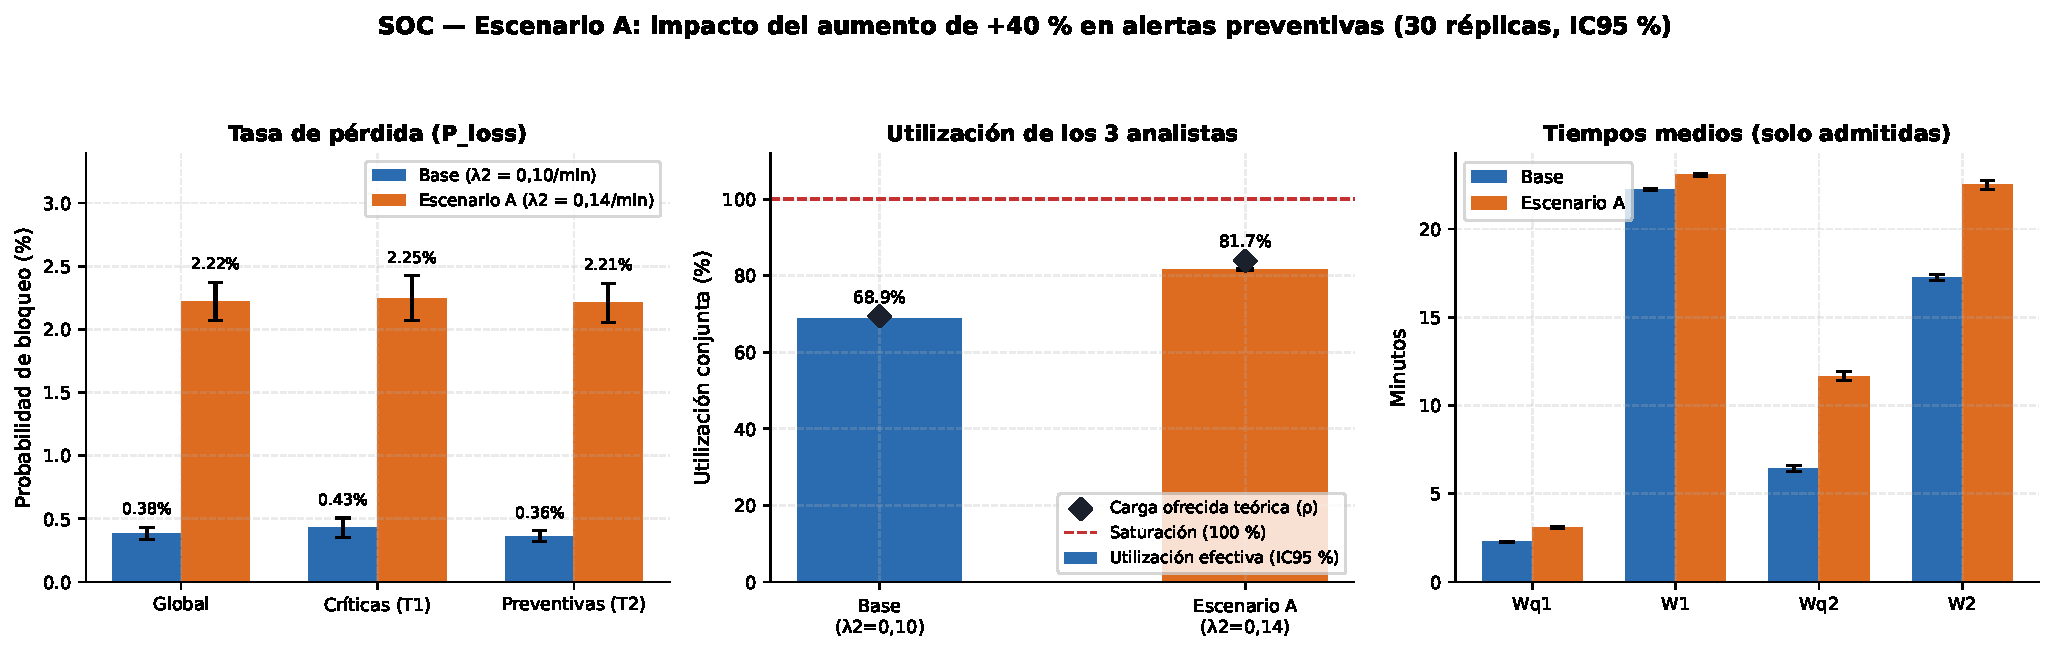
\includegraphics[width=\linewidth]{soc_scenario_a.pdf}
\caption{Escenario A: pérdida de alertas, utilización y tiempos medios frente al caso base.}
\label{fig:escenario-a}
\end{figure}

\subsection{Respuesta a la gerencia}

\textbf{¿En qué porcentaje aumenta la probabilidad de bloqueo?} La
probabilidad de bloqueo global pasa de $0{,}385$\,\% a $2{,}220$\,\%. El
aumento absoluto es $+1{,}835$ puntos porcentuales, con un intervalo de
confianza del 95\,\% de $[1{,}701;1{,}969]$ puntos. En términos relativos, el
aumento es del $477{,}0$\,\% (aproximadamente $5{,}8$ veces la pérdida base).
La pérdida de alertas críticas también crece: pasa de $0{,}431$\,\% a
$2{,}246$\,\% ($+421{,}6$\,\%), aunque las críticas siguen teniendo prioridad
sobre las preventivas.

\textbf{¿Se saturan los tres analistas?} No se alcanza la saturación teórica
al $100$\,\%: la carga ofrecida es $\rho_{\text{ofrecida}}=0{,}8389<1$ y la
utilización efectiva medida es $81{,}65$\,\%. Sin embargo, el sistema opera
mucho más cerca de su límite y la congestión crece de forma no lineal. La
espera media de las preventivas sube de $6{,}42$ a $11{,}66$ minutos
($+81{,}8$\,\%), la de las críticas de $2{,}27$ a $3{,}07$ minutos
($+35{,}6$\,\%) y la cola media de $0{,}750$ a $1{,}741$ alertas
($+132{,}1$\,\%). En consecuencia, aunque los analistas no estén saturados en
sentido teórico, la calidad del servicio se deteriora de forma severa y la
pérdida de alertas críticas se vuelve un riesgo de auditoría.
